\subsection{Overall program structure}
The control flow starts in \texttt{main.c} as usual, and data acquisition happens in \texttt{main.c}. As previously mentioned, all arrays with data (\texttt{afterLowPass}, \texttt{filteredData}..) are stored in a struct called \texttt{data}. When the data is filtered, \texttt{main} calls the filter functions in \texttt{filters.c}; the filter functions return integers that \texttt{main} then stores in \texttt{data}. \\
\\
In contrast, peak detection is invoked by \texttt{main} through the void function \texttt{peakDetection}. In \texttt{qsr.c}, \texttt{peakDetection} begins the chain of functions that carry out the QRS algorithm outlined in chapter \ref{sx:QRSalg}. These function directly alter the variables in \texttt{data}: the doubles \texttt{THRESHOLD1} and \texttt{THRESHOLD2}, the array \texttt{RecentRR} etc. \\
\\
User input is kept at a minimum, but \texttt{qsr.c} invokes several warnings, as outlined in the \textit{Output} chapter. 

\begin{figure}[H]
    \centering
    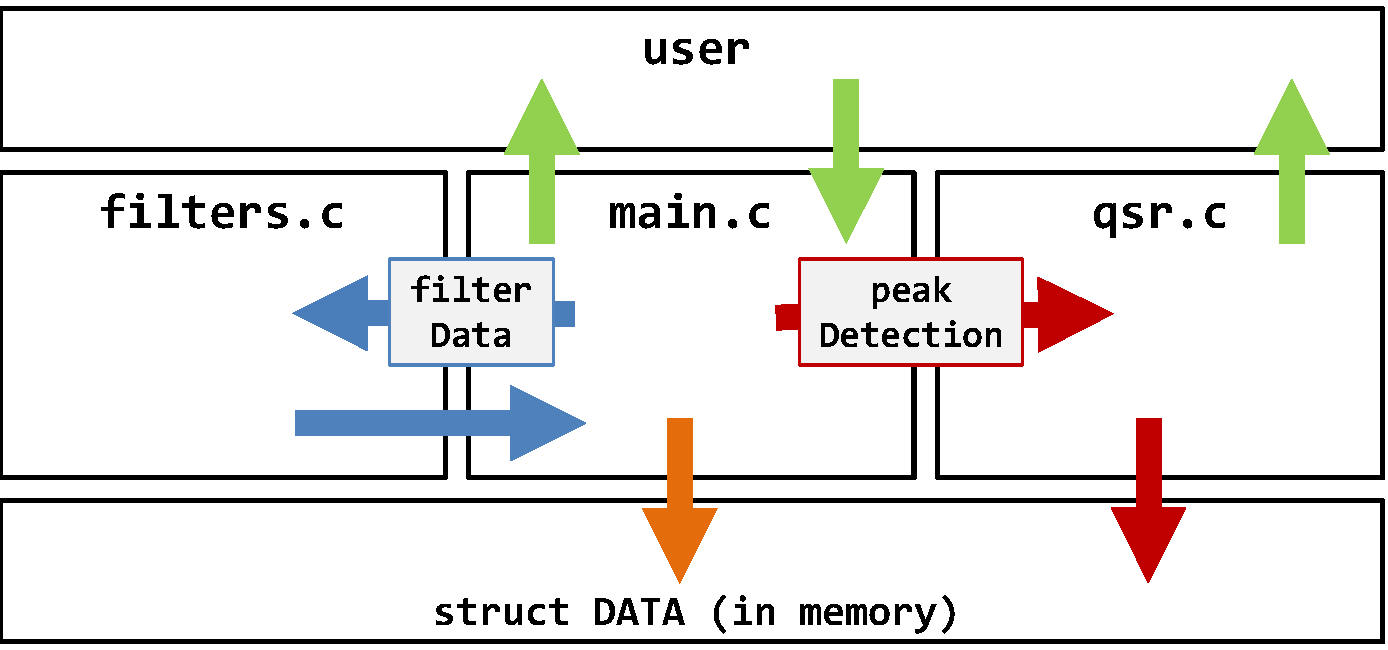
\includegraphics[width=1.0\textwidth]{2Implementation/fig/overall_program_structure.pdf}
    \caption{Overall program structure. \texttt{main.c} handles data acquisition, invokes data filtering, and saves filtered data to a struct. When invoked, \texttt{qsr.c} performs peak detection and saves data to the same struct.}
    \label{fig:overall_program_structure}
\end{figure}

